\documentclass[]{article}
%\documentclass[11pt,a4paper]{article}

%format
\usepackage[utf8]{inputenc}
\usepackage[T1]{fontenc}
\usepackage[english]{babel}
%\usepackage[margin=2.5cm]{geometry}
%math
\usepackage{amsthm}
\usepackage{amsmath}
\usepackage{amsfonts}
\usepackage{amssymb}
\usepackage{stmaryrd}
\usepackage{nicefrac}
\usepackage{mathtools}
%others
\usepackage{hyperref}
\usepackage{graphicx}

%environments
\newtheorem*{remark}{Remark}
\newtheorem*{notation}{Notation}
\newtheorem*{definition}{Definition}
\newtheorem*{example}{Example}
\newtheorem*{question}{Question}
\newtheorem*{exercise}{Exercise}
\newtheorem*{proposition}{Proposition}
\newtheorem*{property}{Property}
\newtheorem{lemma}{Lemma}[section]
\newtheorem{theorem}{Theorem}[section]
\newtheorem{corollary}{Corollary}[section]
\newtheorem{conjecture}{Conjecture}[section]
%commands
%\newcommand{\name}[num]{definition}
\newcommand{\primes}{\mathbb{P}}
%\newcommand{\P}{\mathbb{P}}
\newcommand{\N}{\mathbb{N}}
\newcommand{\Z}{\mathbb{Z}}
\newcommand{\Q}{\mathbb{Q}}
\newcommand{\D}{\mathbb{D}}
\newcommand{\R}{\mathbb{R}}
\newcommand{\C}{\mathbb{C}}
\newcommand{\F}{\mathbb{F}}
\newcommand{\B}{\mathbb{B}}
\newcommand{\Norm}[2][]{\text{Norm}_{#1}(#2)}
\newcommand{\norm}[2][]{\text{Norm}_{#1}(#2)}
\newcommand{\inner}[2]{\left\langle #1,#2 \right\rangle}
\newcommand{\floor}[1]{\lfloor #1 \rfloor}
\newcommand{\ceil}[1]{\lceil #1 \rceil}
\newcommand{\abs}[1]{| #1 |}
\newcommand{\card}[1]{| #1 |}
\newcommand{\curt}[1]{\sqrt[3]{#1}}
\newcommand{\Ker}[1]{\text{Ker}(#1)}
\newcommand{\Image}[1]{\text{Im}(#1)}
\newcommand{\Rank}[1]{\text{Rank}(#1)}
\newcommand{\Nullity}[1]{\text{Nullity}(#1)}
\newcommand{\Span}[1]{\text{Span}(#1)}
\newcommand{\Trace}[1]{\text{Tr}(#1)}
\newcommand{\Det}[1]{\text{Det}(#1)}
\newcommand{\degree}[1]{\partial #1}
\newcommand{\Pow}[1]{\mathcal{P}(#1)}

%opening
\title{Math Wheels}
\author{Paul Dubois}

\begin{document}
	
	\maketitle
	
	\begin{abstract}
		In this paper, we reinvent the wheels.
	\end{abstract}
	
	\section{Introduction}
	In this first section, we will derive what are the requirements for a wheel to "roll properly".
	
	\subsection{What is a wheel?}
	First, we need to rethink the concept of a wheel.
	What makes a wheel convenient? The fact that it rolls, of course. But other shapes could roll, e.g. a non-circular oval.
	However, on a flat surface, oval wheels would not be convenient.
	The principal reason for this is that the height of the rotation axis would not be constant as the wheel turn.
	
	Thus, we decide to define the requirement for a wheel to "roll properly" to have a rotation axis constant.
	
	Let us define this mathematically:
	We take a general wheel shape given by its (positive) radius for all angles $r(\alpha) \in \R^+ \quad \alpha \in \left[ 0, 2\pi \right[$.
	The shape of the wheel is then define by the closed curve\footnote{Assuming $r$ is smooth and such that $\lim\limits_{\alpha \to 2\pi} r(\alpha)=r(0)$.} $\{ (r(\alpha)\cos(\alpha),r(\alpha)\sin(\alpha)) \mid \alpha \in \left[ 0,2\pi \right] \}$.
	We want to find the curve of the road $\{ (x,h(x)) \mid x \in \R \}$ such that the axis of the wheel has a constant height.
	
	We will take as a convention that the wheel is placed vertically at origin (i.e. at $x=0$) with angle $\alpha=0$.
	So at the beginning, the wheel is placed as follows:
	
	\begin{figure}[h!] 
		\centering
		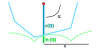
\includegraphics[height=2.7cm]{initial_position}
		\label{fig:InitialPosition}
	\end{figure}
	
	The height of the wheel axis is then $C = h(0)+r(0)$, and we want to keep it constant, i.e. we have the wheel rotation condition:
	
	\begin{equation}
		\tag{Wheel Rotation Condition}
		r(\alpha)+h(x)=C
		\label{eqn:WheelRotationCondition}
	\end{equation}
	
	Note that for the \eqref{eqn:WheelRotationCondition} to be well defined, we need to relate $\alpha$ and $x$.
	
	
	\section{The Wheels Equations}
	Relating $x$ and $\alpha$ is actually the hard part.
	We position our self at angle $\alpha$ corresponding to advance of $x$; and we look at the infinitesimal variation of the road's curve:
	
	\begin{figure}[h!] 
		\centering
		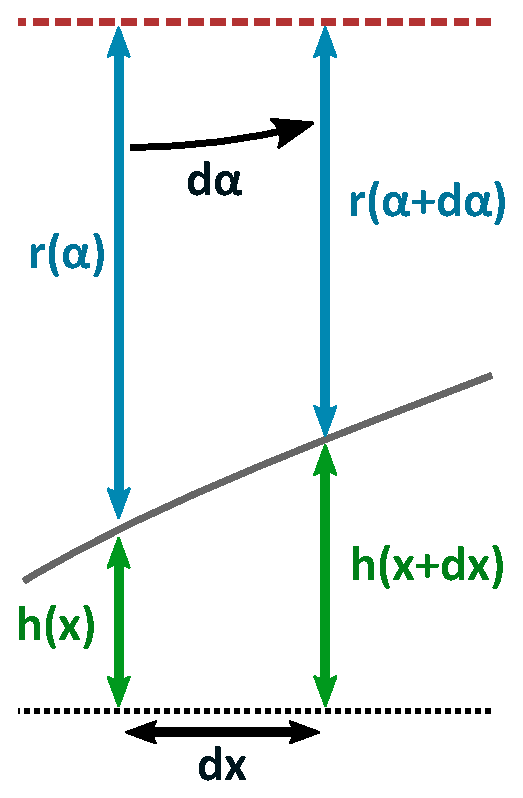
\includegraphics[height=2.7cm]{infinitesimal_scheme}
		\label{fig:infinitesimal_scheme}
	\end{figure}

%	Looking at the problem with intrinsic coordinates, we have:
%	\begin{equation}
%		\tag{Wheel Equations}
%		\left\lbrace 
%		\begin{split}
%			r(\alpha)+h(x)=C\\
%			\tan(a(\alpha)) = \frac{h(x+dx)-h(x)}{dx}\\
%			r(\alpha+d\alpha)+h(x+dx)=C
%		\end{split}
%		\right. 
%		\label{eqn:WheelEquations}
%	\end{equation}



	\subsection{Solving the Wheels Equations}
	
	\section{Collisions}
	\subsection{Local Collisions}
	\subsection{Non-local Collisions}
	
	\section{Conclusion}
	
\end{document}
